% Options for packages loaded elsewhere
\PassOptionsToPackage{unicode}{hyperref}
\PassOptionsToPackage{hyphens}{url}
%
\documentclass[
]{article}
\usepackage{lmodern}
\usepackage{amssymb,amsmath}
\usepackage{ifxetex,ifluatex}
\ifnum 0\ifxetex 1\fi\ifluatex 1\fi=0 % if pdftex
  \usepackage[T1]{fontenc}
  \usepackage[utf8]{inputenc}
  \usepackage{textcomp} % provide euro and other symbols
\else % if luatex or xetex
  \usepackage{unicode-math}
  \defaultfontfeatures{Scale=MatchLowercase}
  \defaultfontfeatures[\rmfamily]{Ligatures=TeX,Scale=1}
\fi
% Use upquote if available, for straight quotes in verbatim environments
\IfFileExists{upquote.sty}{\usepackage{upquote}}{}
\IfFileExists{microtype.sty}{% use microtype if available
  \usepackage[]{microtype}
  \UseMicrotypeSet[protrusion]{basicmath} % disable protrusion for tt fonts
}{}
\makeatletter
\@ifundefined{KOMAClassName}{% if non-KOMA class
  \IfFileExists{parskip.sty}{%
    \usepackage{parskip}
  }{% else
    \setlength{\parindent}{0pt}
    \setlength{\parskip}{6pt plus 2pt minus 1pt}}
}{% if KOMA class
  \KOMAoptions{parskip=half}}
\makeatother
\usepackage{xcolor}
\IfFileExists{xurl.sty}{\usepackage{xurl}}{} % add URL line breaks if available
\IfFileExists{bookmark.sty}{\usepackage{bookmark}}{\usepackage{hyperref}}
\hypersetup{
  pdftitle={Studies of Independent Variables},
  hidelinks,
  pdfcreator={LaTeX via pandoc}}
\urlstyle{same} % disable monospaced font for URLs
\usepackage[margin=0.5cm]{geometry}
\usepackage{color}
\usepackage{fancyvrb}
\newcommand{\VerbBar}{|}
\newcommand{\VERB}{\Verb[commandchars=\\\{\}]}
\DefineVerbatimEnvironment{Highlighting}{Verbatim}{commandchars=\\\{\}}
% Add ',fontsize=\small' for more characters per line
\usepackage{framed}
\definecolor{shadecolor}{RGB}{248,248,248}
\newenvironment{Shaded}{\begin{snugshade}}{\end{snugshade}}
\newcommand{\AlertTok}[1]{\textcolor[rgb]{0.94,0.16,0.16}{#1}}
\newcommand{\AnnotationTok}[1]{\textcolor[rgb]{0.56,0.35,0.01}{\textbf{\textit{#1}}}}
\newcommand{\AttributeTok}[1]{\textcolor[rgb]{0.77,0.63,0.00}{#1}}
\newcommand{\BaseNTok}[1]{\textcolor[rgb]{0.00,0.00,0.81}{#1}}
\newcommand{\BuiltInTok}[1]{#1}
\newcommand{\CharTok}[1]{\textcolor[rgb]{0.31,0.60,0.02}{#1}}
\newcommand{\CommentTok}[1]{\textcolor[rgb]{0.56,0.35,0.01}{\textit{#1}}}
\newcommand{\CommentVarTok}[1]{\textcolor[rgb]{0.56,0.35,0.01}{\textbf{\textit{#1}}}}
\newcommand{\ConstantTok}[1]{\textcolor[rgb]{0.00,0.00,0.00}{#1}}
\newcommand{\ControlFlowTok}[1]{\textcolor[rgb]{0.13,0.29,0.53}{\textbf{#1}}}
\newcommand{\DataTypeTok}[1]{\textcolor[rgb]{0.13,0.29,0.53}{#1}}
\newcommand{\DecValTok}[1]{\textcolor[rgb]{0.00,0.00,0.81}{#1}}
\newcommand{\DocumentationTok}[1]{\textcolor[rgb]{0.56,0.35,0.01}{\textbf{\textit{#1}}}}
\newcommand{\ErrorTok}[1]{\textcolor[rgb]{0.64,0.00,0.00}{\textbf{#1}}}
\newcommand{\ExtensionTok}[1]{#1}
\newcommand{\FloatTok}[1]{\textcolor[rgb]{0.00,0.00,0.81}{#1}}
\newcommand{\FunctionTok}[1]{\textcolor[rgb]{0.00,0.00,0.00}{#1}}
\newcommand{\ImportTok}[1]{#1}
\newcommand{\InformationTok}[1]{\textcolor[rgb]{0.56,0.35,0.01}{\textbf{\textit{#1}}}}
\newcommand{\KeywordTok}[1]{\textcolor[rgb]{0.13,0.29,0.53}{\textbf{#1}}}
\newcommand{\NormalTok}[1]{#1}
\newcommand{\OperatorTok}[1]{\textcolor[rgb]{0.81,0.36,0.00}{\textbf{#1}}}
\newcommand{\OtherTok}[1]{\textcolor[rgb]{0.56,0.35,0.01}{#1}}
\newcommand{\PreprocessorTok}[1]{\textcolor[rgb]{0.56,0.35,0.01}{\textit{#1}}}
\newcommand{\RegionMarkerTok}[1]{#1}
\newcommand{\SpecialCharTok}[1]{\textcolor[rgb]{0.00,0.00,0.00}{#1}}
\newcommand{\SpecialStringTok}[1]{\textcolor[rgb]{0.31,0.60,0.02}{#1}}
\newcommand{\StringTok}[1]{\textcolor[rgb]{0.31,0.60,0.02}{#1}}
\newcommand{\VariableTok}[1]{\textcolor[rgb]{0.00,0.00,0.00}{#1}}
\newcommand{\VerbatimStringTok}[1]{\textcolor[rgb]{0.31,0.60,0.02}{#1}}
\newcommand{\WarningTok}[1]{\textcolor[rgb]{0.56,0.35,0.01}{\textbf{\textit{#1}}}}
\usepackage{graphicx,grffile}
\makeatletter
\def\maxwidth{\ifdim\Gin@nat@width>\linewidth\linewidth\else\Gin@nat@width\fi}
\def\maxheight{\ifdim\Gin@nat@height>\textheight\textheight\else\Gin@nat@height\fi}
\makeatother
% Scale images if necessary, so that they will not overflow the page
% margins by default, and it is still possible to overwrite the defaults
% using explicit options in \includegraphics[width, height, ...]{}
\setkeys{Gin}{width=\maxwidth,height=\maxheight,keepaspectratio}
% Set default figure placement to htbp
\makeatletter
\def\fps@figure{htbp}
\makeatother
\setlength{\emergencystretch}{3em} % prevent overfull lines
\providecommand{\tightlist}{%
  \setlength{\itemsep}{0pt}\setlength{\parskip}{0pt}}
\setcounter{secnumdepth}{-\maxdimen} % remove section numbering

\title{Studies of Independent Variables}
\author{}
\date{\vspace{-2.5em}05.04.2022}

\begin{document}
\maketitle

\hypertarget{bibliotheken-laden-hilfsfunktion}{%
\section{Bibliotheken laden,
Hilfsfunktion}\label{bibliotheken-laden-hilfsfunktion}}

\begin{Shaded}
\begin{Highlighting}[]
\CommentTok{#library(ggplot2)     # moderne plots}
\KeywordTok{library}\NormalTok{(GGally)}

\NormalTok{debug <-}\StringTok{ }\NormalTok{T           }\CommentTok{# debug printout}
\NormalTok{debug <-}\StringTok{ }\NormalTok{F           }\CommentTok{# kein debug printout}
\NormalTok{Log <-}\StringTok{ }\ControlFlowTok{function}\NormalTok{(string) \{}
  \ControlFlowTok{if}\NormalTok{(debug)\{}\KeywordTok{print}\NormalTok{(string)\}  }
\NormalTok{\}}
\end{Highlighting}
\end{Shaded}

\hypertarget{for-all-my-groups}{%
\section{For all MY Groups :}\label{for-all-my-groups}}

\begin{itemize}
\tightlist
\item
  Resistenzen.Rmd generated Resistenzen{[}Schicht{]}.csv, read it in
\item
  plot variables and calculate correlations
\end{itemize}

\begin{Shaded}
\begin{Highlighting}[]
\ControlFlowTok{for}\NormalTok{( Schicht }\ControlFlowTok{in} \KeywordTok{c}\NormalTok{(}\StringTok{"GT8000"}\NormalTok{,}\StringTok{"LE8000"}\NormalTok{,}\StringTok{"U"}\NormalTok{) ) \{     }\CommentTok{# Greater Than 8000 / Less than or Equal to 8000 / Un-stratisfied}
\NormalTok{   FileIn <-}\StringTok{ }\KeywordTok{paste}\NormalTok{( }\StringTok{"Resistenzen"}\NormalTok{,Schicht,}\StringTok{".csv"}\NormalTok{ , }\DataTypeTok{sep=}\StringTok{""}\NormalTok{ )  }
\NormalTok{   Resistenzen <-}\StringTok{ }\KeywordTok{read.csv}\NormalTok{(FileIn)}

  \CommentTok{# csv schreiben fügt vorne Index-Spalte an; diese entfernen :}
\NormalTok{  Resistenzen[,}\DecValTok{1}\NormalTok{] <-}\StringTok{ }\OtherTok{NULL}                      

  \ControlFlowTok{if}\NormalTok{(debug)\{}\KeywordTok{View}\NormalTok{(Resistenzen)\}}

\NormalTok{  df <-}\StringTok{ }\KeywordTok{data.frame}\NormalTok{(}\DataTypeTok{WM.gr  =}\NormalTok{ Resistenzen}\OperatorTok{$}\NormalTok{WM.group,      }\CommentTok{# unabhängige Variablen extrahieren}
                 \DataTypeTok{OLS.gr =}\NormalTok{ Resistenzen}\OperatorTok{$}\NormalTok{OLS.group,     }\CommentTok{# Titel kürzen, sonst Platzprobleme ...}
                 \DataTypeTok{IAC.gr =}\NormalTok{ Resistenzen}\OperatorTok{$}\NormalTok{IAC.group, }
                 \DataTypeTok{HSC.gr =}\NormalTok{ Resistenzen}\OperatorTok{$}\NormalTok{HSC.group,}
                 \DataTypeTok{MY     =}\NormalTok{ Resistenzen}\OperatorTok{$}\NormalTok{MY, }
                 \DataTypeTok{SCC    =}\NormalTok{ Resistenzen}\OperatorTok{$}\NormalTok{SCC, }
                 \DataTypeTok{CBC    =}\NormalTok{ Resistenzen}\OperatorTok{$}\NormalTok{CBC, }
                 \DataTypeTok{DIA    =}\NormalTok{ Resistenzen}\OperatorTok{$}\NormalTok{DIA)}
  \CommentTok{#View(df)}
  \KeywordTok{print}\NormalTok{(}\KeywordTok{ggpairs}\NormalTok{(df, }\DataTypeTok{title =} \KeywordTok{paste}\NormalTok{(}\StringTok{"group:"}\NormalTok{,Schicht)))}
  \KeywordTok{print}\NormalTok{(}\StringTok{""}\NormalTok{)}
\NormalTok{\}}
\end{Highlighting}
\end{Shaded}

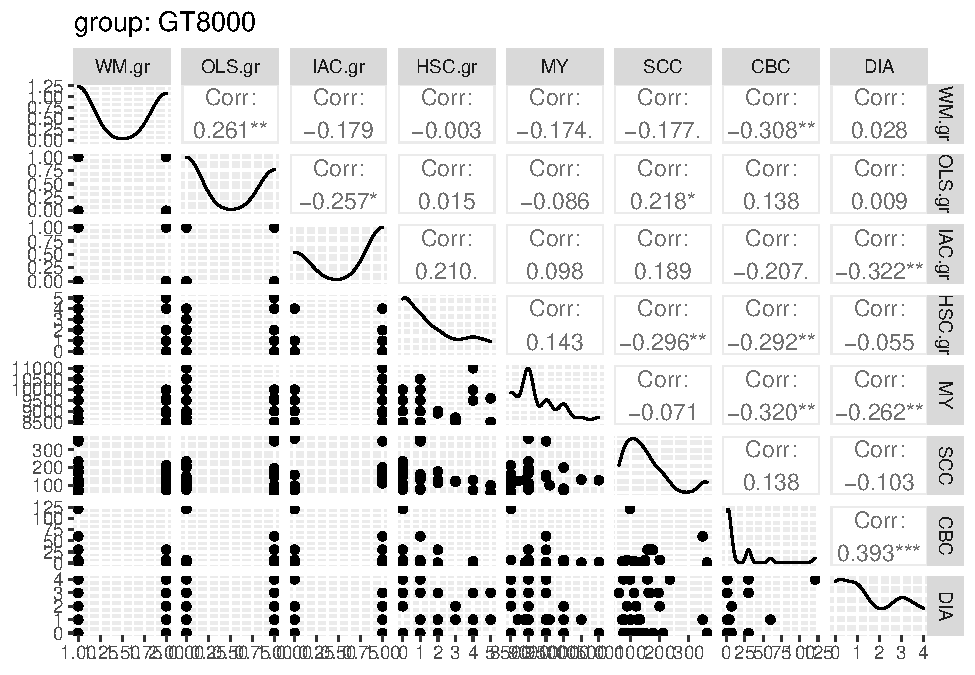
\includegraphics{IndependentVariables_files/figure-latex/unnamed-chunk-2-1.pdf}

\begin{verbatim}
## [1] ""
\end{verbatim}

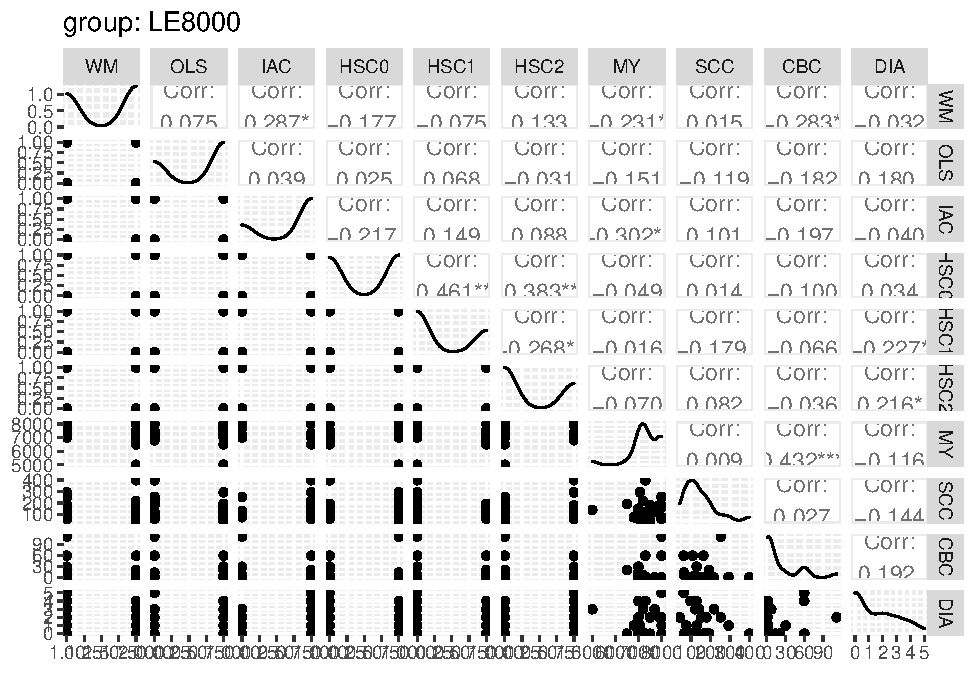
\includegraphics{IndependentVariables_files/figure-latex/unnamed-chunk-2-2.pdf}

\begin{verbatim}
## [1] ""
\end{verbatim}

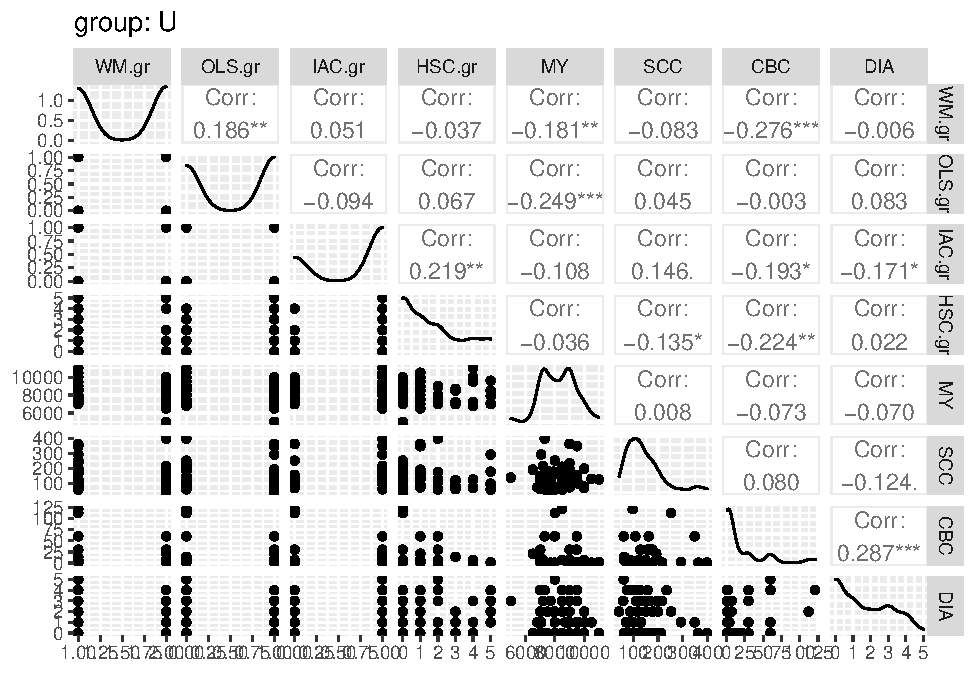
\includegraphics{IndependentVariables_files/figure-latex/unnamed-chunk-2-3.pdf}

\begin{verbatim}
## [1] ""
\end{verbatim}

\hypertarget{linear-depence}{%
\subsection{Linear Depence?}\label{linear-depence}}

As it implies multicollinearity, the logistic regression would be
unreliable in its presence.

The maximum correlation magnitude amounts to

\begin{itemize}
\tightlist
\item
  28.7\% in the unstratisfied analysis
\item
  43.3\% in the stratisfied analysis
\end{itemize}

These are not yet a strong linear correlations, they don't hint to
collinearity problems in the multivariate logistic regression.

\hypertarget{outliers}{%
\subsection{Outliers?}\label{outliers}}

Im wesentlichen sind nur die plots ohne diskrete Variablen gut zu
interpretieren (für die anderen könnte man bessere Grafiken machen,
hätte dann aber immer noch das Problem der beliebigen Kodierung).

In Histogrammen und Streuplots sehe ich einen Ausreisser mit MY = 5000,
das ist Farm 32. Ist sie als problematisch bekannt?

\end{document}
